%  !TeX  root  =  user_guide.tex

\section{从这里开始}\label{label_getstarted}

% when the revision of a section has been finalized, 
% comment out the following line:
% \updatedisclaimer

本章对 \qg 的安装, \qg 网页的一些样本数据以及使栅格和矢量图层首次在一个简单的对话框中显示进行了概述。

\section{安装}\label{label_installation}
\index{installation}

\qg 非常容易安装。标准安装程序包可在MS Windows和Mac OSX操作系统中运行。并且我们提供了许多GNU/Linux特色的二进制安装包(rpm和deb格式)或者可以软件包管理器直接安装的软件仓库。 \qg 主页 \url{http://qgis.osgeo.org/download/} 上提供了二进制安装包的最新消息。

\minisec{从源代码安装}

如果你需要从源代码编译 \qg ,请参阅网址 \url{http: //qgis.osgeo.org/documentation/} 可用的编码和编制指南。  \qg 的源代码中也附有安装说明。

\minisec{从外部介质安装}

\qg 允许用户指明 --configure 选项来覆盖原本默认的用户配置文件目录(例如,Linux下面可能是 ~/.qgis),并且让Qt设置QSettings也使用该目录。这样做可以,例如,使得在闪存介质上安装使用 \qg 软件及插件并保存设置成为可能。

\section{示例数据}\label{label_sampledata}
\index{data!sample} 

用户指南中包含了许多基于 \qg 示例数据集的例子。
\win Windows安装程序中有一个可以下载 \qg 示例数据集的选项。选中它的话,安装程序会下载示例数据到 \filename{My Document}目录下的 \filename{GIS Database}目录内。用户可以使用Windows资源管理器将此文件夹移动到任何方便的位置。如果用户在初始安装 \qg 软件时并没有选中安装样本数据集的复选框,也可以通过以下方式完成:

\begin{itemize}[label=--]
\item 使用已有的GIS数据;
\item 从 \qg 网站 \url{http://qgis.osgeo.org/download} 上下载示例数据; 
\item 如果以上方法不成功的话,你还可以卸载 \qg 并重新安装,同时选中下载数据选框。
\end{itemize}

\nix \osx 对于GNU/Linux和Mac OSX操作系统,目前还没有rpm、deb或dmg格式的数据集安装包。要使用示例数据就需要从网站 \url{http://download.osgeo.org/qgis/data/} 下载ZIP或者TAR格式的压缩文件 \filename{\qg\_sample\_data} 并将其解压缩到您的系统当中。阿拉斯加数据集中包含了用户指北所有例子和截图使用的全部GIS数据,还包含一个小型的GRASS数据库。 \qg 示例数据集的投影为阿拉斯加地区的艾博斯等积投影(Alaska Albers Equal Area),单位是英尺,投影的EPSG代码是2964。

\begin{verbatim}
PROJCS["Albers Equal Area",
    GEOGCS["NAD27",
        DATUM["North_American_Datum_1927",
            SPHEROID["Clarke 1866",6378206.4,294.978698213898,
                AUTHORITY["EPSG","7008"]],
            TOWGS84[-3,142,183,0,0,0,0],
            AUTHORITY["EPSG","6267"]],
        PRIMEM["Greenwich",0,
            AUTHORITY["EPSG","8901"]],
        UNIT["degree",0.0174532925199433,
            AUTHORITY["EPSG","9108"]],
        AUTHORITY["EPSG","4267"]],
    PROJECTION["Albers_Conic_Equal_Area"],
    PARAMETER["standard_parallel_1",55],
    PARAMETER["standard_parallel_2",65],
    PARAMETER["latitude_of_center",50],
    PARAMETER["longitude_of_center",-154],
    PARAMETER["false_easting",0],
    PARAMETER["false_northing",0],
    UNIT["us_survey_feet",0.3048006096012192]]
\end{verbatim}

如果用户想用 \qg 做为GRASS的图形前端,可在GRASS GIS官方网站 \url{http://grass.osgeo.org/download/data.php} 搜索下载示例地区的数据集合,例如斯皮尔菲什(Spearfish)或南达科他州(South Dakota)。

\section{示例会话}\label{samplesession}

在安装了 \qg 并且下载了示例数据之后,我们可以示范一个简单的示例会话:对一个栅格或者矢量图层进行可视化显示。我们将使用一个土地利用的栅格图层 \filename{\qg\_sample\_data/raster/landcover.img} 和一个湖泊的矢量图层\filename{\qg\_sample\_data/gml/lakes.gml} 。

\minisec{启动 \qg}

\begin{itemize}[label=--]
\item \nix{在命令提示符下键入 \qg ,或者若使用预编译的二进制程序的话使用应用程序菜单来启动 \qg 。}
\item \win{用开始菜单或桌面快捷方式或者双击 \qg 工程文件打开 \qg 。}
\item \osx{双击应用程序文件夹中的图标。}
\end{itemize} 

\begin{figure}[ht]
   \centering 
   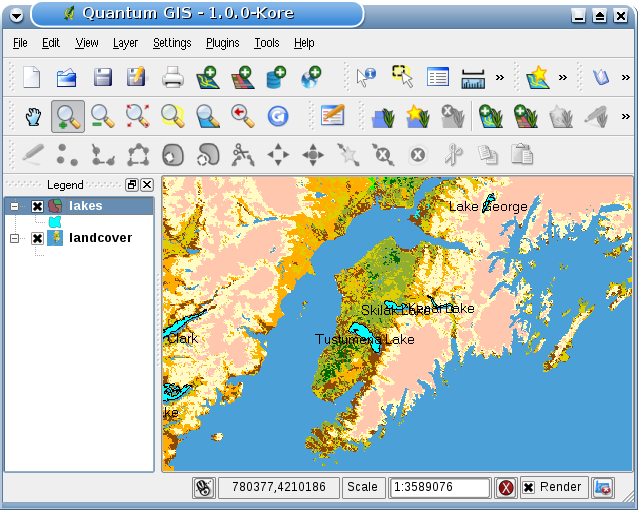
\includegraphics[clip=true, width=12cm]{simple_session}
   \caption{一个简单的 \qg 会话示例 \nixcaption}\label{fig:simple_session}
\end{figure}

\minisec{装载样本示例集中的栅格和矢量图层}

{\setlength{\baselineskip}{1.3\baselineskip}
\begin{enumerate}[itemsep=2pt]

\item 点击 \toolbtntwo{mActionAddRasterLayer}{Load Raster} 图标。 
\item 浏览 \filename{\qg\_sample\_data/raster/} 目录,选择ERDAS图像文件 \filename{landcover.img}并点击 \button{打开}。
\item 如果该文件没有列出,请检查在对话框底部的文件类型组合框的类型设置是否正确。在这个例子中应选择“Erdas Imagine Images (*.img, *.IMG)”。
\item 现在点击 \toolbtntwo{mActionAddOgrLayer}{加载矢量图层} 。 
\item 在弹出的 \dialog{添加矢量图层}对话框中,将“源类型”设置为 \radiobuttonon{文件} 。然后单击 \button{浏览} ,选择目标图层。
\item 定位至 \filename{\qg\_sample\_data/gml/} 目录下,在文件类型组合框中选择“GML”,然后选择 \filename{lake.gml} 并点击 \button{打开},然后在添加矢量图层对话框中点击 \button{确定}。
\item 把最喜欢的湖泊区域放大一点。
\item 在地图图例上双击 \filename{lakes} 图层以打开 \dialog{图层属性} 对话框。
\item 点击 \tab{符号} 标签页并选择蓝色作为填充颜色。
\item 点击 \tab{标注} 标签页并选中 \checkbox{显示标注} 复选框以启用标注。选择“NAMES”字段作为标注来源字段。
\item 为了提高标注的可读性,您可以在标注文字周围添加一个白色的缓冲区:在列表左侧点击“缓冲区”,选中 \checkbox{标注缓冲区?} ,缓冲区大小设置为3。
\item 点击 \button{应用},查看显示结果是否理想,最后点击 \button{确定}。
\end{enumerate} 
\par}
现在您发现了在 \qg 中可视化显示栅格和矢量图层是多么的简单吧。接下来的一章会介绍更多的功能特性、设置方法以及如何来更好地使用 \qg 。

\FloatBarrier
